%%%%%%%%%%%%%%%%%%%%%%%%%%%%%%%%%%%%%%%%%
% 2016SoE020
% IGERT Symposium
% Portland State University
% Seot 2016
% slides begin line 207
% %%%%%%%%%%%%%%%%%%%%%%%%%%%%%%%%%%%%%%%

%----------------------------------------------------------------------------------------
%	PACKAGES AND OTHER DOCUMENT CONFIGURATIONS
%----------------------------------------------------------------------------------------
% The class {scrartcl} pro­vides the “ar­ti­cle”-like el­e­ment of the koma-script col­lec­tion.
% The doc­u­ment lay­out of the class is less ‘stri­dent’ than that of ar­ti­cle, and it of­fers 
% much more flex­i­bil­ity than ar­ti­cle via other el­e­ments of the koma-script col­lec­tion. 
% https://www.ctan.org/pkg/scrartcl?lang=en
% https://www.ctan.org/topic/class
\documentclass[
paper=128mm:96mm, % The same paper size as used in the beamer class
fontsize=11pt, % Font size
pagesize, % Write page size to dvi or pdf
parskip=half-, % Paragraphs separated by half a line
]{scrartcl} 

\linespread{1.12} % Increase line spacing for readability

%--------- Required packages
\usepackage{xcolor}	 % Required for custom colors
% Define a few colors for making text stand out within the presentation
% Use these colors within the presentation by enclosing text in the commands below
\definecolor{mygreen}{RGB}{44,85,17}
\definecolor{myblue}{RGB}{34,31,217}
\definecolor{mybrown}{RGB}{194,164,113}
\definecolor{myred}{RGB}{255,66,56}
\newcommand*{\mygreen}[1]{\textcolor{mygreen}{#1}}
\newcommand*{\myblue}[1]{\textcolor{myblue}{#1}}
\newcommand*{\mybrown}[1]{\textcolor{mybrown}{#1}}
\newcommand*{\myred}[1]{\textcolor{myred}{#1}}
\usepackage[includeheadfoot,
top=3.5mm,
bottom=3.5mm,
left=5.5mm,
right=5.5mm,
headsep=6.5mm,
footskip=8.5mm
]{geometry} % Page margins settings

\usepackage[T1]{fontenc}	 % Fonts, for correct hyphenation and T1 encoding
\usepackage{lmodern}         % Default font: latin modern font
	%\usepackage{fourier} % Alternative font: utopia
	%\usepackage{charter} % Alternative font: low-resolution roman font
\renewcommand{\familydefault}{\sfdefault} % Sans serif - this may need to be commented to see the alternative fonts
\usepackage{amsmath}
\usepackage{amsthm} % Required for theorem environments
\usepackage{bm} % Required for bold math symbols (used in the footer of the slides)
\usepackage{graphicx} % Required for including images in figures
\usepackage{booktabs} % Required for horizontal rules in tables
\usepackage{multicol} % Required for creating multiple columns in slides
\setlength{\columnsep}{0.1mm}
\usepackage{lastpage} % For printing the total number of pages at the bottom of each slide
\usepackage[english]{babel} % Document language - required for customizing section titles
\usepackage{microtype} % Better typography
\usepackage{tocstyle} % Required for customizing the table of contents
\usepackage{caption}
\captionsetup{labelformat=empty,labelsep=none}
\usepackage{mathtools}
\usepackage{subcaption}
\usepackage{nicefrac}
\usepackage{csquotes}
\usepackage{enumitem}	%spread enumeration over multiple slides
\usepackage{pdfpages}
\usepackage{tikz}  
\usepackage[absolute, overlay]{textpos} %position textblocks (absolute) on the page
\setlength{\TPHorizModule}{\textwidth}
\setlength{\TPVertModule}{\textwidth}
\usepackage{scrpage2} % Slide layout configuration; Required for customization of the header and footer
\pagestyle{scrheadings} % Activates the pagestyle from scrpage2 for custom headers and footers
\clearscrheadfoot % Remove the default header and footer
\setkomafont{pageheadfoot}{\normalfont\color{black}\sffamily} % Font settings for the header and footer
\usepackage{titlesec} % Required for customizing section spacing; deeper section titles are given less space due to lesser importance
\titlespacing{\section}{0mm}{0mm}{0mm} % Lengths are: left, before, after
\titlespacing{\subsection}{0mm}{0mm}{-1mm} % Lengths are: left, before, after
\titlespacing{\subsubsection}{0mm}{0mm}{-2mm} % Lengths are: left, before, after
\setcounter{secnumdepth}{0} % How deep sections are numbered, set to no numbering by default - change to 1 for numbering sections, 2 for numbering sections and subsections, etc

% Presentation mode (uncomment for full screen)
%\usepackage{hyperref} 
%\hypersetup{pdfpagemode=FullScreen}



%---------- Sets vertical centering of slide contents with increased space between paragraphs/lists
\makeatletter
\renewcommand*{\@textbottom}{\vskip \z@ \@plus 1fil}
\newcommand*{\@texttop}{\vskip \z@ \@plus .5fil}
\addtolength{\parskip}{\z@\@plus .25fil}
\makeatother

%----------- Remove page numbers and the dots leading to them from the outline slide
\makeatletter
\newtocstyle[noonewithdot]{nodotnopagenumber}{\settocfeature{pagenumberbox}{\@gobble}}
\makeatother
\usetocstyle{nodotnopagenumber}

%-------- Change the name of the table of contents
\AtBeginDocument{\renewcaptionname{english}{\contentsname}{\Large Outline}} 


%---------- Header configuration
\ihead{
\hspace{-2mm}
\begin{tikzpicture}[remember picture,overlay]
\node [xshift=\paperwidth/2,yshift=-\headheight] (mybar) at (current page.north west)[rectangle,fill,inner sep=0pt,minimum width=\paperwidth,minimum height=2\headheight,top color=mygreen!64,bottom color=mygreen]{}; % Colored bar
\node[below of=mybar,yshift=3.3mm,rectangle,shade,inner sep=0pt,minimum width=128mm,minimum height =1.5mm,top color=black!50,bottom color=white]{}; % Shadow under the colored bar
shadow
\end{tikzpicture}
\color{white}\runninghead} % Header text defined by the \runninghead command below and colored white for contrast

%------------- Footer configuration
	%\newlength{\footheight}
\setlength{\footheight}{8mm} % Height of the footer
\addtokomafont{pagefoot}{\footnotesize} % Small font size for the footnote
% Left side footer
\ifoot{
\hspace{-2mm}
\begin{tikzpicture}[remember picture,overlay]
\node [xshift=\paperwidth/2,yshift=\footheight] at (current page.south west)[rectangle,fill,inner sep=0pt,minimum width=\paperwidth,minimum height=3pt,top color=mygreen,bottom color=mygreen]{}; % Green bar
\end{tikzpicture}
\vspace{-3.5 mm}
\myauthor\ {$\bm{\vert}$}\ \myuni % Left side text
%\myauthor\ \raisebox{-0.5mm}{$\bm{\vert}$}\ \myuni % Left side text
}
% Right side footer
\ofoot[\pagemark/\pageref{LastPage}\hspace{-2mm}]{\pagemark/\pageref{LastPage}\hspace{-2mm}} 



%----------- Specialty new commands
% Paragraph indent
\newenvironment{myindentpar}[1]%
   {\begin{list}{}%
       {\setlength{\leftmargin}{#1}}%
           \item[]%
   }
     {\end{list}}
     
% Theorem style
\newtheoremstyle{mythmstyle} % Defines a new theorem style used in this template
{0.5em} % Space above
{0.5em} % Space below
{} % Body font
{} % Indent amount
{\sffamily\bfseries} % Head font
{} % Punctuation after head
{\newline} % Space after head
{\thmname{#1}\ \thmnote{(#3)}} % Head spec
	
\theoremstyle{mythmstyle} % Change the default style of the theorem to the one defined above
\newtheorem{theorem}{Theorem}[section] % Label for theorems
\newtheorem{remark}[theorem]{Remark} % Label for remarks
\newtheorem{algorithm}[theorem]{Algorithm} % Label for algorithms
\makeatletter % Correct qed adjustment


% The code for the box which can be used to highlight an element of a slide (such as a theorem)
\newcommand*{\mybox}[2]{ % The box takes two arguments: width and content
\par\noindent
\begin{tikzpicture}[mynodestyle/.style={rectangle,draw=mygreen,thick,inner sep=2mm,text justified,top color=white,bottom color=white,above}]
\node[mynodestyle,at={(0.5*#1+2mm+0.4pt,0)}]{ % Box formatting
\begin{minipage}[t]{#1}
#2
\end{minipage}
};
\end{tikzpicture}
\par\vspace{-1.3em}}

% Arrow over vector
\newcommand{\amsvect}{%
  \mathpalette {\overarrow@\vectfill@}}
\def\vectfill@{\arrowfill@\relbar\relbar{\raisebox{-3.81pt}[\p@][\p@]{$\mathord\mathchar"017E$}}}

% Nice-looking fractions
\newcommand\ddfrac[2]{\frac{\displaystyle #1}{\displaystyle #2}}


%----------------------------------------------------------------------------------------
%	PRESENTATION INFORMATION
%----------------------------------------------------------------------------------------
% Title
\newcommand*{\mytitle}{Agricultural-Ecological Mutualism: \\
 Feeding People and Planet}
% Running head displayed on almost all slides
\newcommand*{\runninghead}{Agricultural-ecological mutualism}
% Presenters name(s)
\newcommand*{\myauthor}{bmarron} 
% Presentation date
\newcommand*{\mydate}{20 Sept 2016} 
% University or department
\newcommand*{\myuni}{
\includegraphics[scale=.30]{graphics2/psulogo_horiz_msword.eps}} 



%#############
%SLIDES
%#############
\begin{document}

%slide1 (Title slide) ------------------------------------------------------------
\thispagestyle{empty} % No slide header and footer

\begin{tikzpicture}[remember picture,overlay] % Background box
	%\node [xshift=\paperwidth/2,yshift=\paperheight/2] at (current page.south west)[rectangle,fill,inner
\node [xshift=\paperwidth/2,yshift=7 cm] at (current page.south west)[rectangle,fill,inner sep=0pt,minimum width=\paperwidth,minimum height=\paperheight/3,top color=mygreen,bottom color=mygreen]{};
\end{tikzpicture}

% Text within the tikz box
\begin{flushright}
\vspace{-2.7cm}
\color{white}
\sffamily{\bfseries\normalsize\mytitle\par} % Title
\vspace{.1cm}
\normalsize
\myauthor\par % Author name
\vspace{-.3cm}
\mydate\par % Date
%\vfill
\end{flushright}
 \hspace*{2cm}
 \vspace*{-2cm}
\clearpage


%slide2----------------------------------------------------------

\begin{tikzpicture}[overlay]
  \node[anchor=south west] at (3,-5.5) {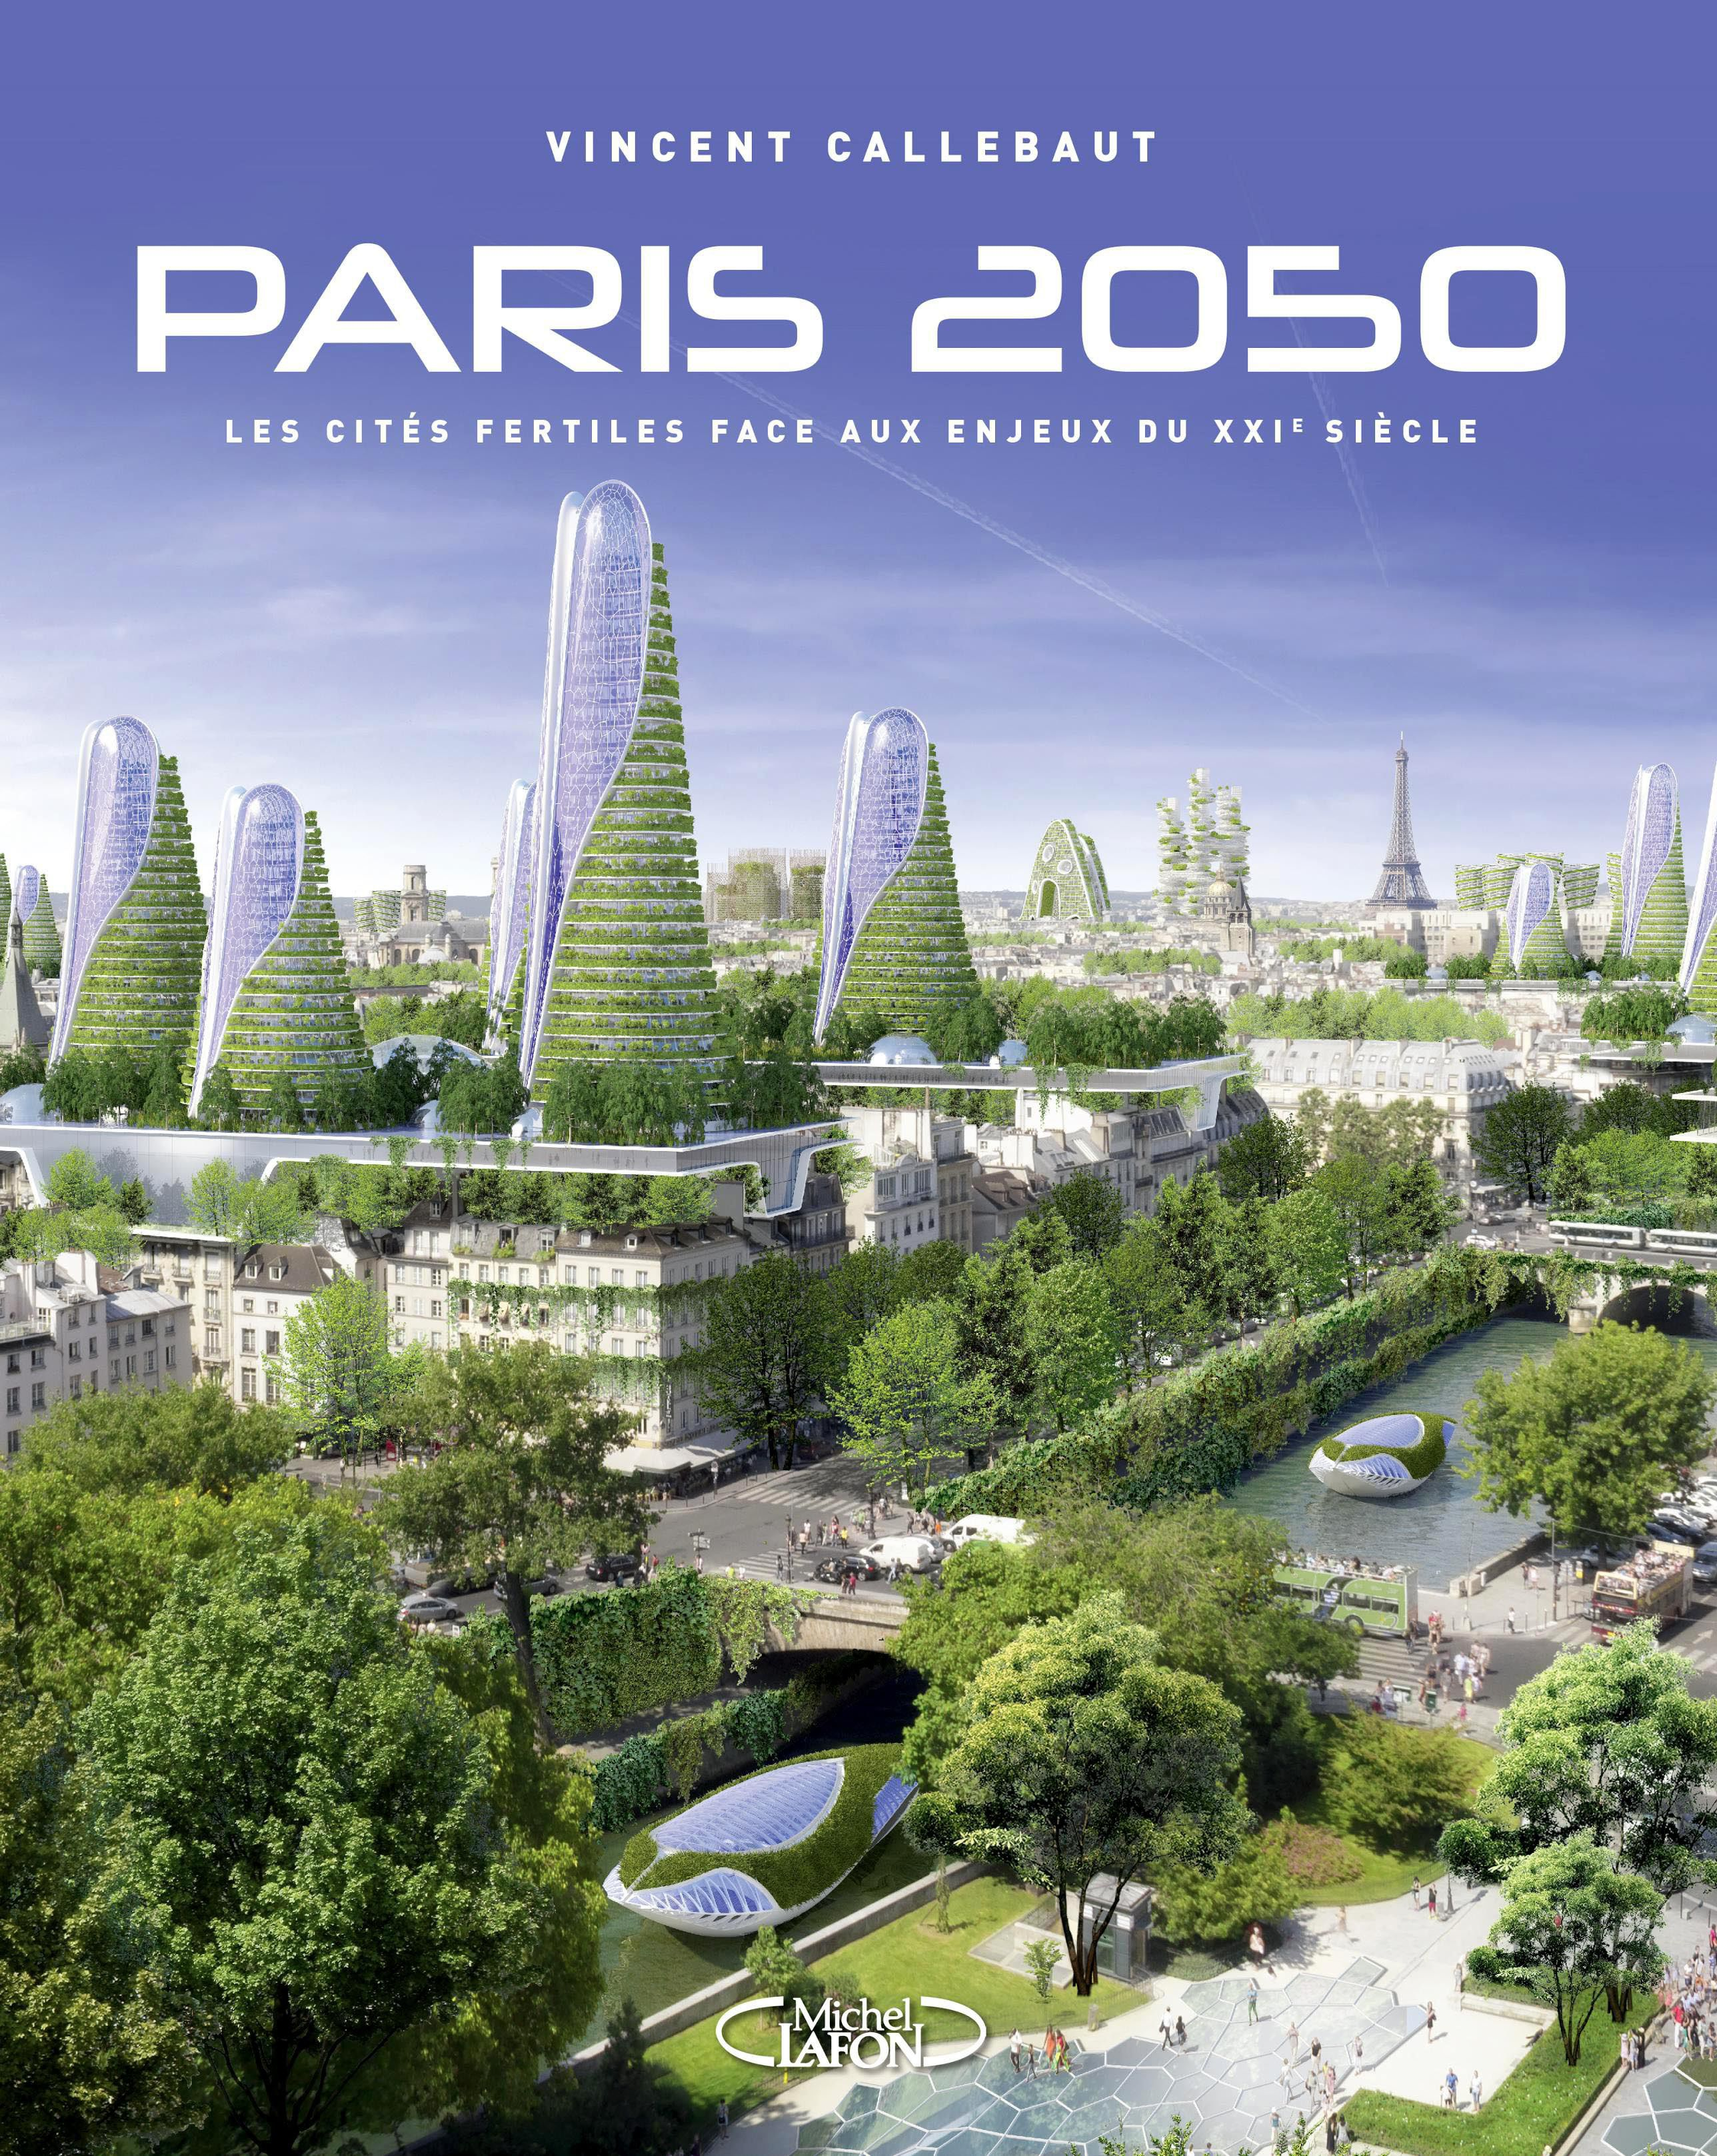
\includegraphics[scale=.06]{graphics1/fig1a}};  
 \end{tikzpicture}
 
\clearpage


%slide3----------------------------------------------------------

\begin{tikzpicture}[overlay]
  \node[anchor=south west] at (1.3,-5.5) {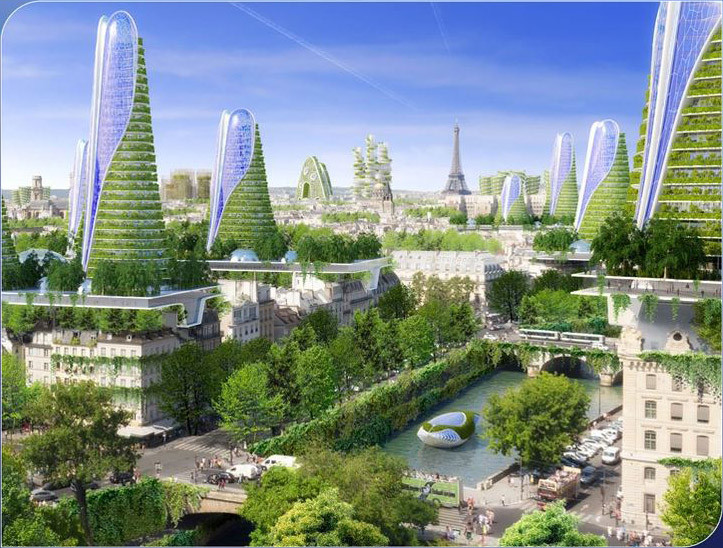
\includegraphics[scale=.50]{graphics1/fig1b}};
 \end{tikzpicture}
 
\clearpage


%slide4----------------------------------------------------------

\begin{tikzpicture}[overlay]
  \node[anchor=south west] at (1.2,-5.5) {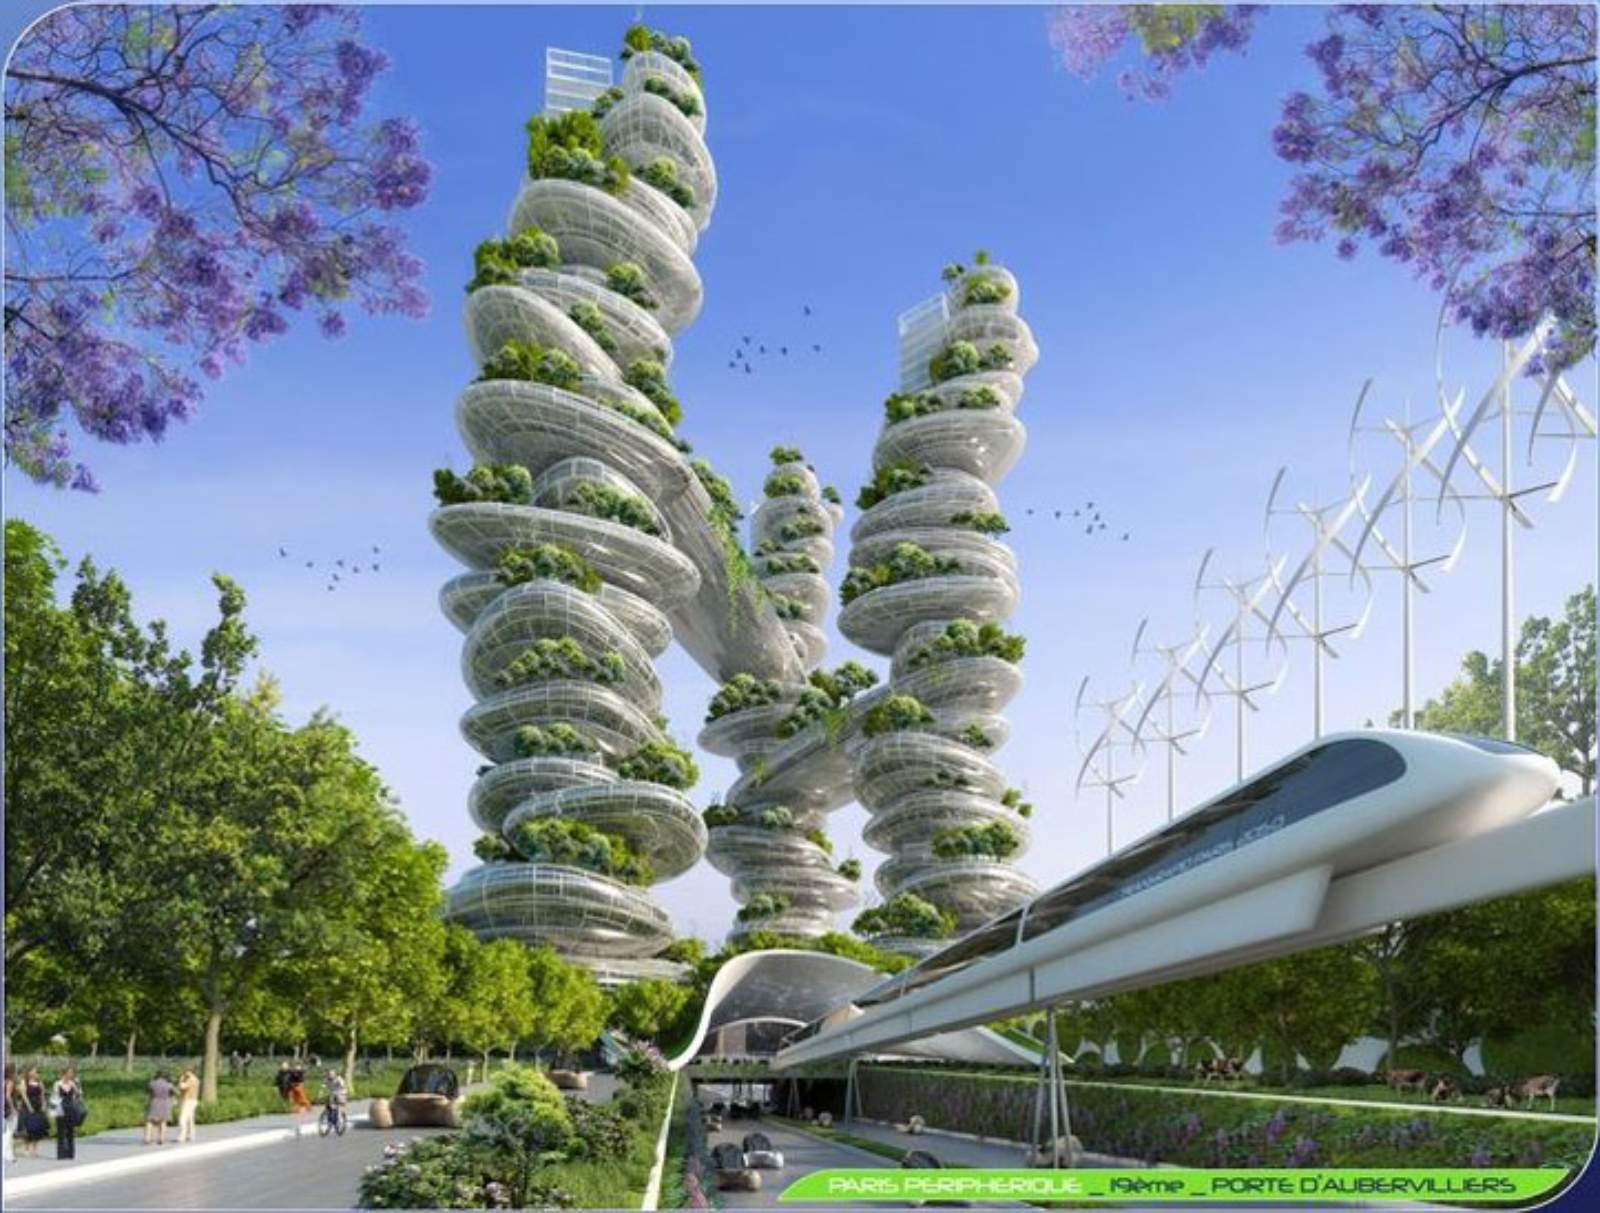
\includegraphics[scale=.17]{graphics1/fig1c}};
 \end{tikzpicture}
 
\clearpage


%slide5----------------------------------------------------------

\begin{tikzpicture}[overlay]
  \node[anchor=south west] at (.55,-5.5) {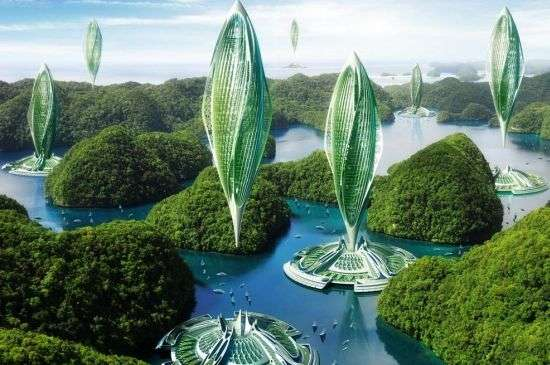
\includegraphics[scale=.55]{graphics1/fig2}};
 \end{tikzpicture}
 
\clearpage


%slide6----------------------------------------------------------

\begin{tikzpicture}[overlay]
  \node[anchor=south west] at (.75,-5) {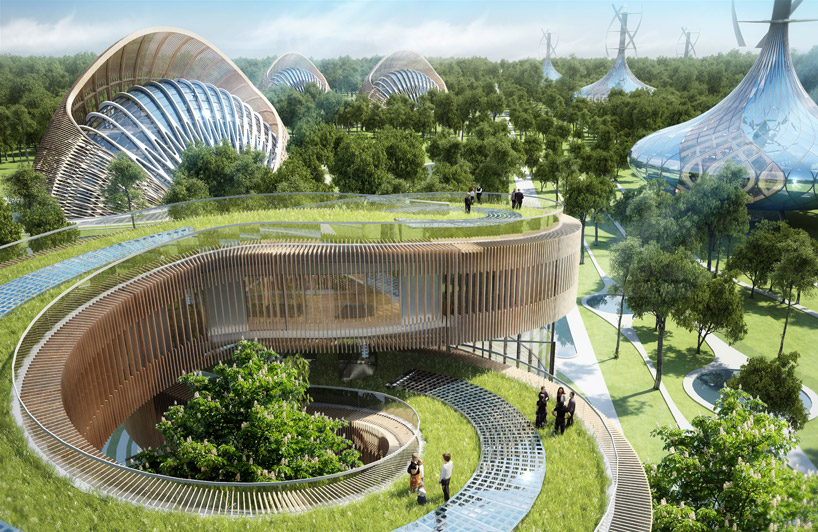
\includegraphics[scale=.35]{graphics1/fig3}};
 \end{tikzpicture}
 
\clearpage



%slide7----------------------------------------------------------

\begin{tikzpicture}[overlay]
  \node[anchor=south west] at (.75,-5.4) {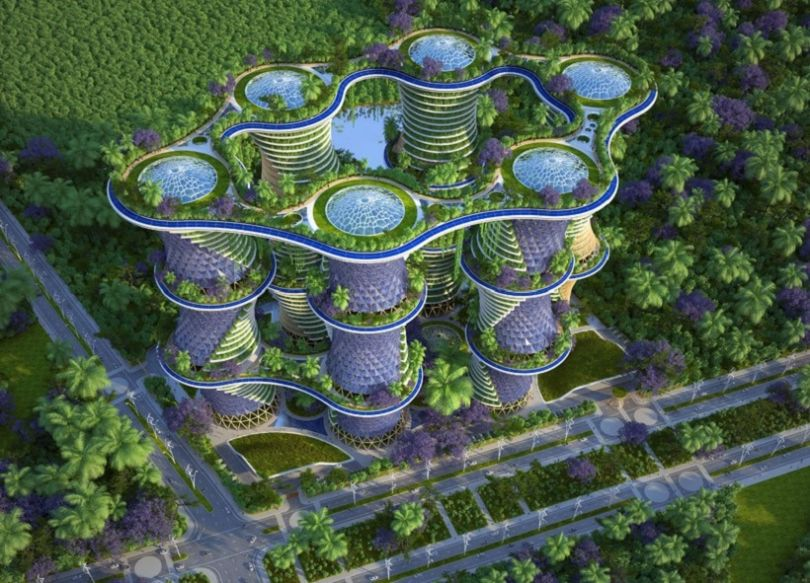
\includegraphics[scale=.45]{graphics1/fig4}};
 \end{tikzpicture}
 
\clearpage


%slide8----------------------------------------------------------

\begin{tikzpicture}[overlay]
  \node[anchor=south west] at (3,-5.4) {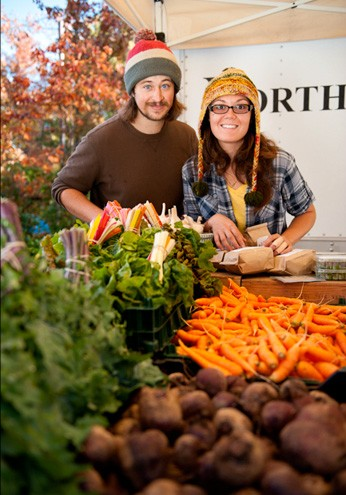
\includegraphics[scale=.4]{graphics1/fig6}};
 \end{tikzpicture}
 
\clearpage


%slide9----------------------------------------------------------

\begin{tikzpicture}[overlay]
  \node[anchor=south west] at (3,-5.4) {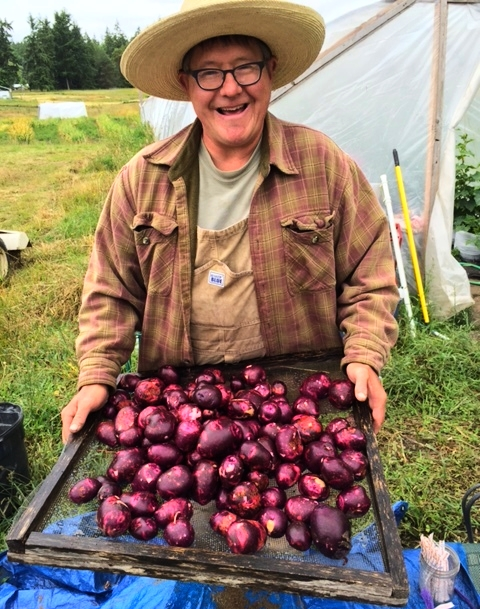
\includegraphics[scale=.4]{graphics1/fig7}};
 \end{tikzpicture}
 
\clearpage


%slide10----------------------------------------------------------

\begin{tikzpicture}[overlay]
  \node[anchor=south west] at (1,-5) {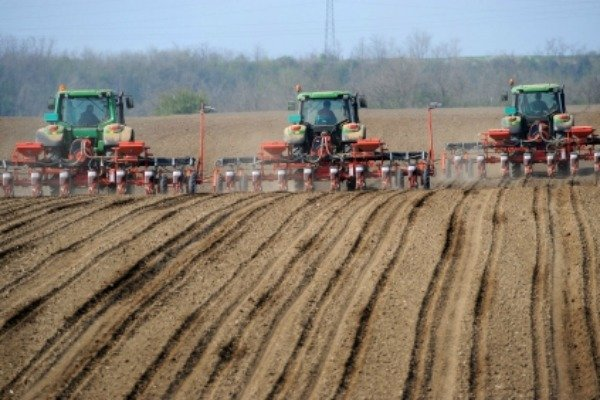
\includegraphics[scale=.45]{graphics1/fig8}};
 \end{tikzpicture}
 
\clearpage


%slide11----------------------------------------------------------

\begin{tikzpicture}[overlay]
  \node[anchor=south west] at (1.5,-5) {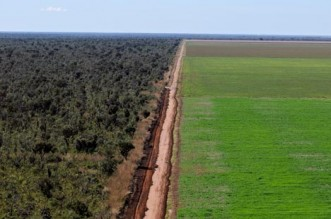
\includegraphics[scale=.75]{graphics1/fig9}};
 \end{tikzpicture}
 
\clearpage


%slide12----------------------------------------------------------

\begin{tikzpicture}[overlay]
  \node[anchor=south west] at (1.5,-5) {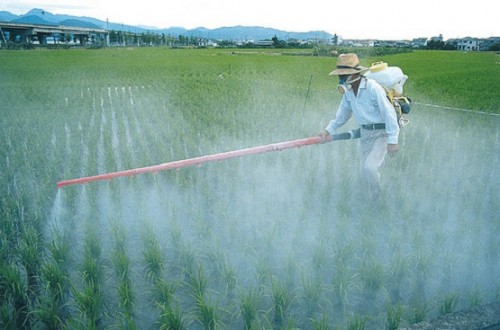
\includegraphics[scale=.5]{graphics1/fig10}};
 \end{tikzpicture}
 
\clearpage


%slide13----------------------------------------------------------

\begin{tikzpicture}[overlay]
  \node[anchor=south west] at (.05,-5) {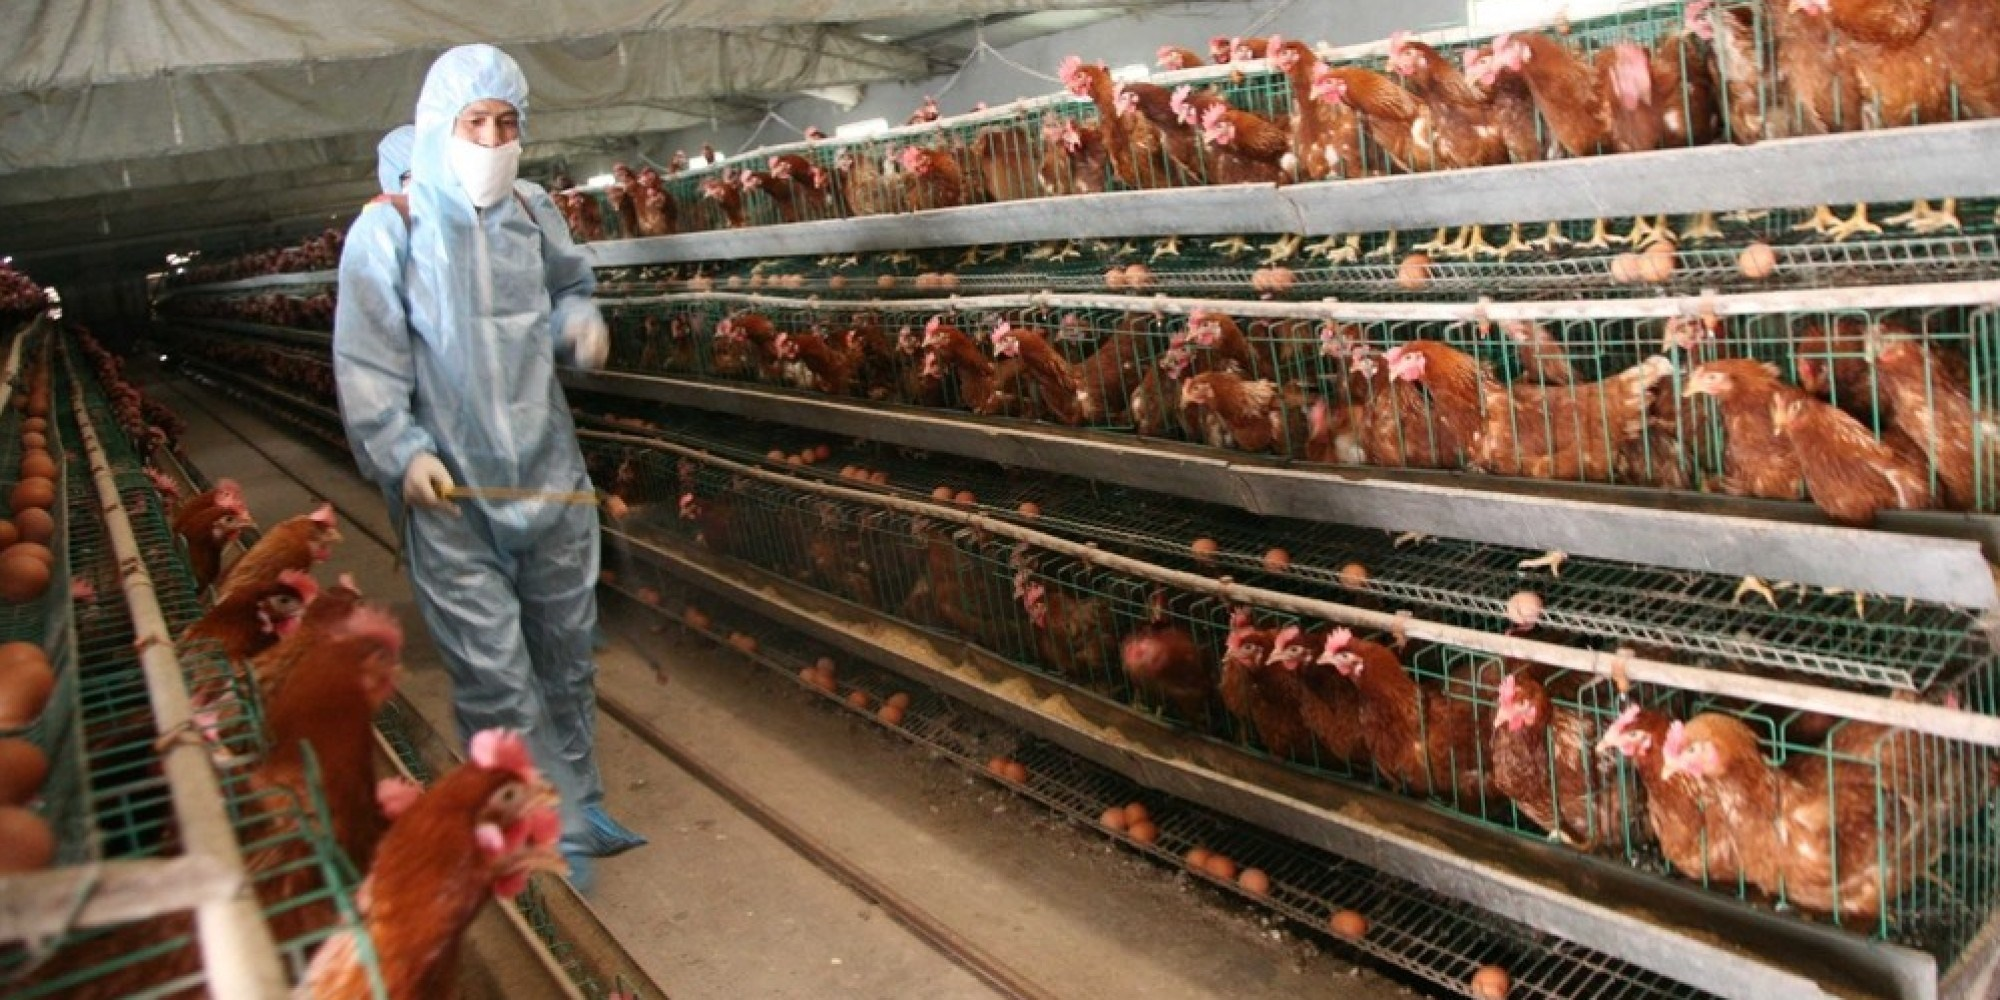
\includegraphics[scale=.165]{graphics1/fig11}};
 \end{tikzpicture}
 
\clearpage

%slide 14a--------------------------------------------------------------
\subsection{from the US Congress...}
\footnotesize {
Sec. 3103. Definitions.\\
(19) The term \enquote{sustainable agriculture} means an integrated system of plant and animal production
practices having a site-specific application that will, over the long-term-\\
(A) satisfy human food and fiber needs;\\
(B) enhance environmental quality and the natural resource base upon which the agriculture economy
depends;\\
(C) make the most efficient use of nonrenewable resources and on-farm resources and integrate, where
appropriate, natural biological cycles and controls;\\
(D) sustain the economic viability of farm operations; and\\
(E) enhance the quality of life for farmers and society as a whole.\\
7 U.S.C. Sec. 3103(19)
}

\clearpage



%slide 14b-----------------------------------------

\subsection{Important Questions}    
\begin{itemize}
\item How can we design low-impact, low-input, robust, sustainable food production systems at the landscape scale that simultaneously maximize regional agricultural and ecological productivity? Is agricultural-ecological mutualism possible?
\item Why do some agro-ecological practices work and some don't?
\item Can virtuous agricultural and ecological cycles be generated by \enquote*{tuning} landscape scale disturbance regimes like agriculture?
\item What is the parsimonious set of state variables required to adequately assess the degree of agricultural-ecological mutualism for different agro-ecological landscape patterns?
\end{itemize}
\clearpage


%slide15-----------------------------------------
\begin{textblock}{1}(.1,.16)
\textbf{Agricultural-ecological mutualism} -- the set of complex linkages and relationships \\
that provide for mutually beneficial transfers of matter, energy, and information \\
between the agriculturally-organized and the naturally-organized components of a \\
multi-functional landscape.
\end{textblock}

\begin{tikzpicture}[overlay]
  \node[anchor=south west] at (2,-5) {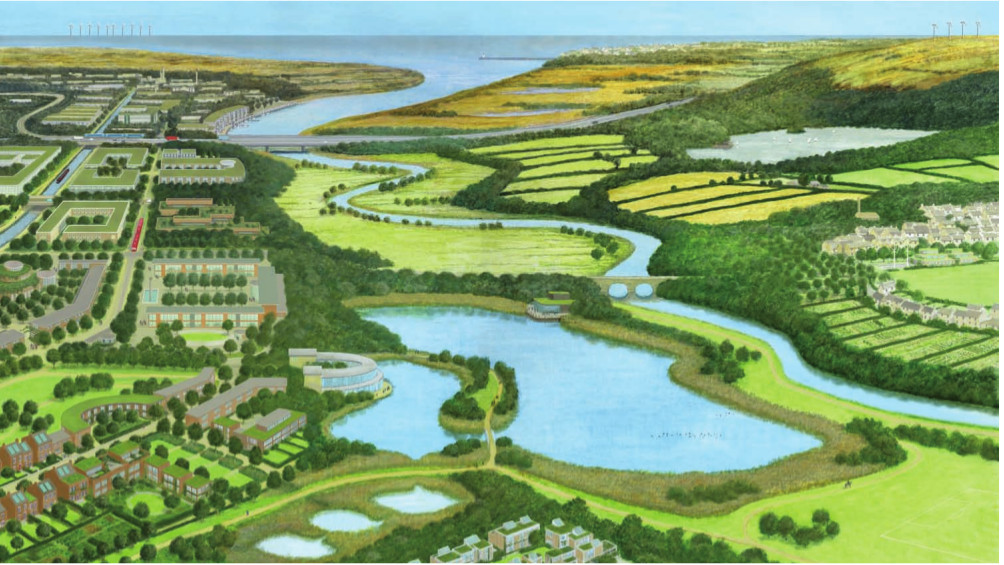
\includegraphics[scale=.3]{graphics1/fig15}};
 \end{tikzpicture}
 
 \begin{textblock}{1}(.23,.71)
  \small {(The Landscape Institute, 2016)}
 \end{textblock}

\clearpage



%slide16-----------------------------------------

\begin{tikzpicture}[overlay]
  \node[anchor=south west] at (1.5,-4) {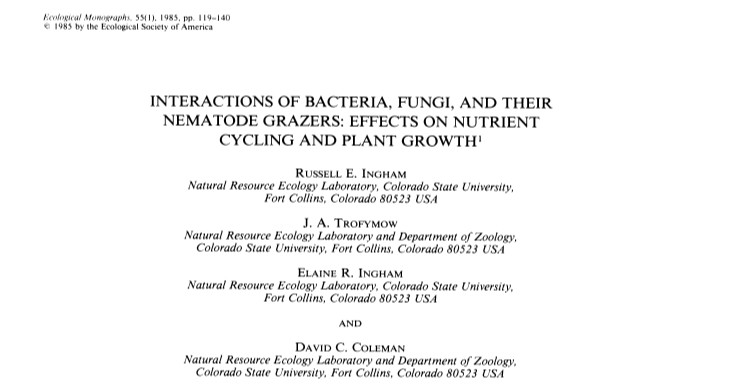
\includegraphics[scale=.5]{graphics1/fig12c}};
 \end{tikzpicture}

\clearpage


%slide17-----------------------------------------

\begin{tikzpicture}[overlay]
  \node[anchor=south west] at (.5,-1) {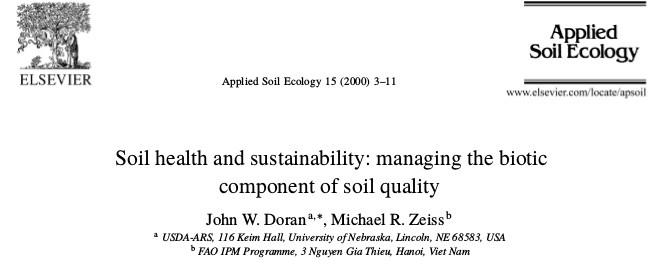
\includegraphics[scale=.35]{graphics1/fig12b}};
  \node[anchor=south west] at (.5,-2.1) {
\includegraphics[scale=.35]{graphics1/fig12e}};
  \node[anchor=south west] at (.5,-4.5) {
\includegraphics[scale=.35]{graphics1/fig12g}};
  \node[anchor=south west] at (7,-2) {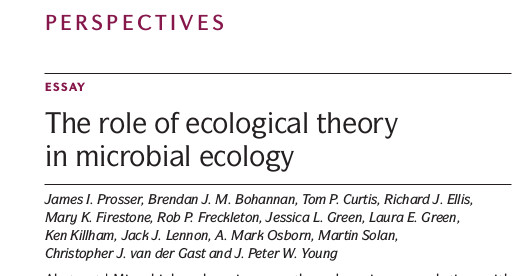
\includegraphics[scale=.35]{graphics1/fig12f}};
 \end{tikzpicture}

\clearpage


%slide 17a------------------------------------
\begin{tikzpicture}[overlay]
  \node[anchor=south west] at (1.5,-5.5) {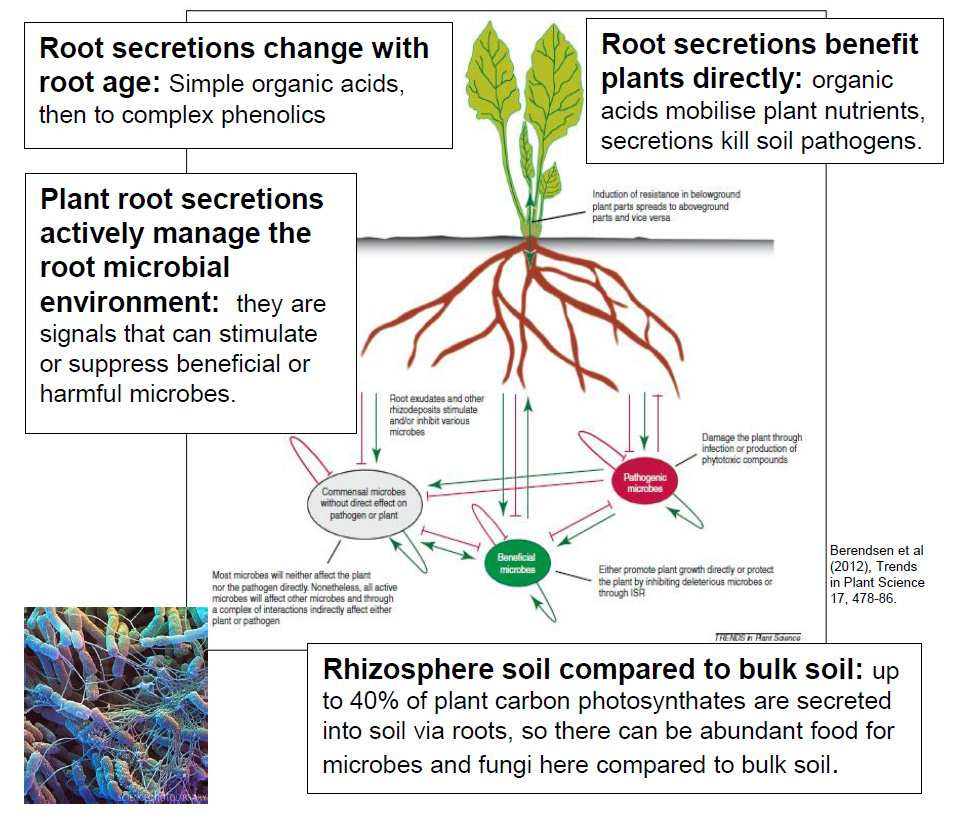
\includegraphics[scale=.25]{graphics1/fig16}};
 \end{tikzpicture}

\clearpage

%slide18-----------------------------------------

\begin{tikzpicture}[overlay]
  \node[anchor=south west] at (.5,-5.75) {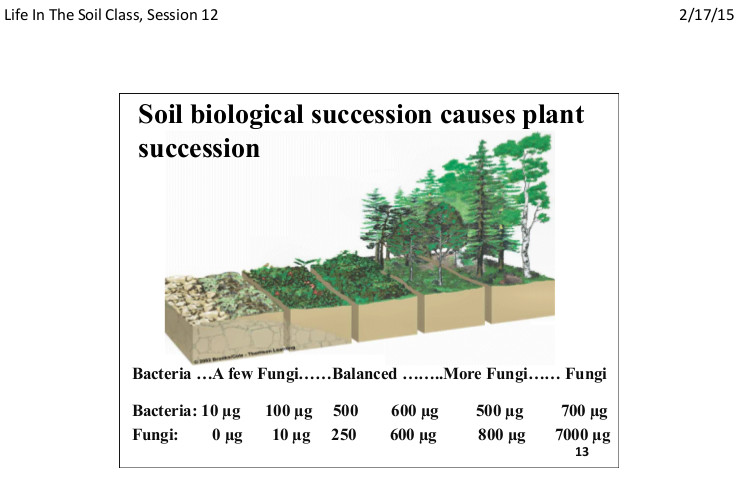
\includegraphics[scale=.6]{graphics1/fig13}};
 \end{tikzpicture}

\begin{textblock}{1}(.1,.16)
  \footnotesize {(Ingham, 2015)}
 \end{textblock}
\clearpage


%slide19-----------------------------------------

\begin{tikzpicture}[overlay]
  \node[anchor=south west] at (.5,-5) {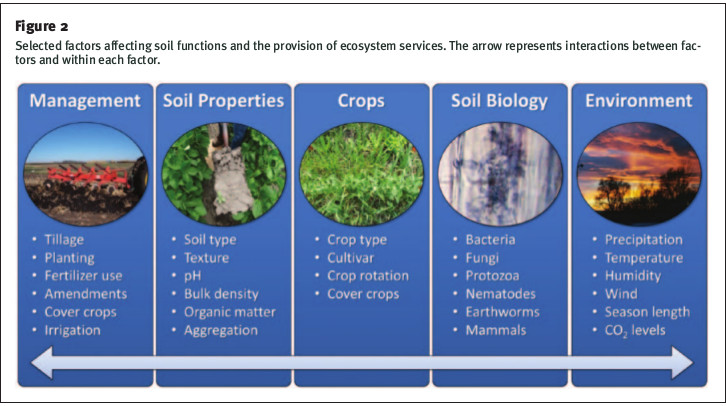
\includegraphics[scale=.6]{graphics1/fig14}};
 \end{tikzpicture}
 
 \begin{textblock}{1}(.1,.7)
  \small {(Lehman et al., 2015)}
 \end{textblock}

\clearpage

%slide20-----------------------------------------
\subsubsection{Soil food web typologies may provide the theoretical as well as the applied basis for agricultural-ecological mutualism. }
\textit{\underline{If} it is the energetic (trophic) and biochemical transformations brokered by rhizospheric fungal/bacterial/protozoa assemblages that are primarily responsible for soil nutrient cycling \underline{and} there are readily identifiable rhizospheric fungal/bacterial/protozoa assemblages fueled by root exudates that constitute functional soil food webs, \underline{then} different natural successional stages should have unique soil food webs \underline{and} outcomes of interactions in the rhizosphere should ultimately affect plant and soil community dynamics at the ecosystem scale \underline{and} maximizing the nutrient retention (SOM) and trophic energy capture capabilities of any given landscape may require a set of successionally derived, soil food webs.}

\clearpage

%slide21------------------------------------------------
\subsubsection{Next steps in my research agenda}    
\begin{enumerate}
	\item Assessment of soil food web typologies by field sampling (optical microscopy) for the major successional stages of successionally developed agroecosystems in the Yucat\'an Peninsula of Mexico.
	\item Correlation of soil food web typologies to agricultural and ecological productivity using literature-derived data and the Yucat\'an field sample data.
	\item Construction of a LANDIS-II model of a successionally developed agroecosystem.
	\item Experimentation with the LANDIS-II model to evaluate ANPP of various agroecological landscape patterns driven by coupled, agricultural and ecosystem disturbance regimes.
\end{enumerate}






\end{document}
